\chapter{Porting TinyOS for Chronos hardware}

This chapter describes the work done to make TinyOS run on Chronos watch. Firstly, we show how we added a minimal, yet functional, platform to the OS. Then, we discuss the methodology used for introducing new code and go over a basic MCU configuration, which is fundamental for the operation of other systems. Afterwards, we present a conceptual schema of the watch circuits that, most notably, shows connections between the hardware components. The remainder part of the chapter describes the hardware drivers we have created, starting with the MCU internal systems and going towards the peripherals.

\section{Adding a minimal functional platform}

The first milestone of our project, was to get to the point, where we could compile the \emph{Null} application and upload its image to the watch. Although this application is of little use, it does basic system initialization. Therefore, it allows for verifying the build configuration. The additional benefit was that we could learn the TinyOS build process.

To compile code for the MSP430 architecture, we used \emph{\bf msp430-gcc}. This was an obvious choice, because the NesC compiler has a built-in support for \emph{gcc}. Its installation wasn't, however, as easy as one might expect. Namely packages provided in Ubuntu were too old and did not contain headers for the \emph{CC430F6137} MCU. In the end, we removed all related system packages and built \emph{msp430-gcc} from sources, using the most recent version available at the time: 4.6.2.  In addition to the compiler, tools like \emph{msp430-gdb} and \emph{mspdebug} were also installed.

The \emph{\bf mspdebug} tool is particularly important for Chronos development, as it allows for flashing software on the watch through the USB debug dongle.  Additionally, it allows for debugging code running on the watch: it provides a primitive gdb server, to which \emph{msp430-gdb} is able to connect\footnote{It's imperative to use the most recent version of \emph{msp430-gdb}, because older versions are not compatible with the \emph{mspdebug} tool.}.

Afterwards, the {\bf NesC compiler} was installed from sources as well. Then we choose and installed a clean upstream version of the TinyOS, provided by \cite{TOSnet}. It contained some tools and scripts and we installed those too.

At that point, we had a functional TinyOS installation, capable of targeting MSP430-based boards, like \emph{telosb}. We choose to name the new platform for our watch as \emph{chronos}. To make if fully functional, we had to create a few files under the \emph{tos/platforms/chronos} path, among which only \emph{.platform} was non-trivial. This configuration file holds various compilation parameters, in particular, the exact MCU model used in the watch, so that the generated binary images get correct offsets for the code segment (0x8000) and the interrupt vector (0xFF80).

We also wanted the build process of an application to be initiated with a standard TinyOS make command:
\begin{lstlisting}[numbers=none, language=bash]
  $ make chronos install
\end{lstlisting}
For this to work, we had to add a configuration file under the \emph{tos/support/make} path. The \emph{chronos.target} file adds our platform to the build system, which in turn takes care of the exact NesC compiler invocations. In addition, file \emph{mspdebug.extra} was added under the \emph{tos/support/make/msp} path, which invokes the commands that program Chronos.

These changes may seem obvious, but it took us quite some time to work them out. Eventually, we reached a point where the \emph{Null} application was successfully installed on the watch.

\section{Code creation methodology}

The next step was to add code that would make the watch operational. Generally it's considered a good programming practice to reuse existing code rather than write it from scratch. Existing code tends to be more tested and can save considerable time, especially when it contains nontrivial constructions that would otherwise require a test and debug cycle to discover. Such situations are especially frequent when dealing with hardware. Moreover, our project was quite time constrained from the beginning and various delays were to be expected further on. Under those circumstances, saving time wherever possible was particularly important. We benefited greatly from the fact that TinyOS code licensing is very liberal, allowing for free use, with few reasonable restrictions, like preserving the license headers in files.

Nevertheless, not all goals could be completed by adapting existing components. In cases where no drivers in NesC were available, we had to fall back to the hardware documentation in the form of datasheets. They describe hardware's behaviour well, though sometimes certain issues were only discovered and compensated for after the driver code was implemented and run. As a rule, documentation is low level, describing only control registers available on the device. All higher-layer  abstraction had to be devised and implemented by us. This was a tedious task and applying the Hardware Abstraction Architecture eased it enormously. We didn't know that from the beginning, though. Therefore, some designs follow it better than others. Besides, in practice boundaries between layers aren't always clear.

A few times we encountered code that was close to what we needed, but some hardware differences precluded using it directly. Modifications had to be done before it could be added to the Chronos platform. In those cases, we had to mix the above approaches by studying the datasheets to understand the inner workings of the code. However, we found that both contributed to better understanding. Code told us much about the inner workings of the hardware and datasheets helped understanding the constructions used in the code. Most notably, such an approach was used to port the low level radio driver, but the principle extends to other components. As a rule, it was much easier to understand the operation of a hardware device if, even a crude, driver implementation was available.

To implement the code, we first used traditional terminal based tools, like the \emph{vim} editor. Later on, when we discovered the \emph{Yetti 2} plugin (see Appendix \ref{ch:prog_env}), we started using \emph{Eclipse} with all its benefits. This increased our productivity considerably. Moreover, there is no emulator of the watch available. Therefore, all testing had to be done by uploading images to the hardware and observing its responses. At first, we didn't even know if programming was successful, but when the LCD display became available, followed by the serial console, and ultimately visual debugger, the process became quite seamless. See Appendix \ref{ch:prog_env} for details.

Finally, in what we believe is \emph{the way} to create code for mobile platforms, we tried to use \emph{TOSMOCK} for module unit-testing. This technology, however, became available too late to be widely used in our code.

\section{MCU configuration}

The MCU configuration was made much easier, thanks to the existence of a partial port of TinyOS to a similar hardware platform. The Texas Instruments \cite{EM430}, shown in Figure~\ref{fig:em430_board}, is a development board which uses the exact same \emph{CC430F6137} MCU chip as Chronos does. Work on the port was done as a part of the \cite{OSIAN} project. Even though Chronos and EM430 differ in peripherals, much of the internal MCU configuration code was compatible and we decided to reuse it.  Minor modifications were required to meet our coding standards and, to fix a few issues.
\begin{figure}[h]
  \centering
  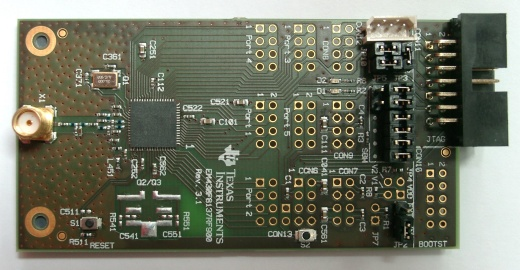
\includegraphics[width=0.65\textwidth]{img/em430_board.jpg}
  \caption{The Texas Instruments EM430F6137RF900.}
  \label{fig:em430_board}
\end{figure}

The entire MCU configuration is done in the \emph{PlatformC} and \emph{PlatformP} components, shown in Figure~\ref{fig:platformc}.
\begin{figure}[h]
  \centering
  \includegraphics[width=1.0\textwidth]{diagrams/platformc.eps}
  \caption{\emph{PlatformC} performs MCU initialization.}
  \label{fig:platformc}
\end{figure}
The first step that \emph{PlatformP} takes is disabling the watchdog timer. Otherwise, the timer would shortly reset the device. Disabling the timer requires only a single register assignment and is done inline. In the future, we may wish to use the watchdog to increase Chronos's reliability, but it wasn't a priority in this stage of the project.

\subsection{Millisecond timers}

One of the primary MCU responsibilities is providing clocks and timing for other subsystems. Let's first look at timers. In Section \ref{ch:timer_subsystem}, we introduced TinyOS timer library stating that \emph{HilTimerMilliC} is provided by each platform. Continuing that discussion, Figure~\ref{fig:hil_timer_milli_c} shows a simplified structure of this component, as it is provided by the \emph{chronos} platform.
Let's explain its operation in a bottom-up order.
\begin{figure}[h!]
  \centering
  \includegraphics[width=0.55\textwidth]{diagrams/hil_timer_milli_c.eps}
  \caption{Structure of Chronos's \emph{HilTimerMilliC}. (simplified)}
  \label{fig:hil_timer_milli_c}
\end{figure}

The \emph{Msp430Timer32khzC} gives access to one of the hardware timers. \emph{Msp430AlarmC} uses it to provide an \emph{Alarm} interface with a 32kHz granularity and a 16-bit range. Then, it is transformed by \emph{TransformAlarmC} into a wider 32 bit alarm with 1ms (actually $10^6 / 2^{10} \approx 976.5\upmu$s) granularity. Finally, this alarm is converted into a timer and virtualized. Note that these transforming components all come from the TinyOS library.

\subsection{Microsecond alarms}

The millisecond granularity isn't, however, sufficient for some of the Chronos peripheral drivers. Where delays on the order of microseconds are needed we didn't want to resort to active waiting. Having latency and memory footprint in mind, we decided to implement virtualized 16-bit microsecond alarms\footnote{Note, that microsecond timing is quite imprecise. Firstly it's difficult to get an event fired within 10$\upmu$s and the exact firing time can vary by as much as 25$\upmu$s. Still, if a 37$\upmu$s delay is necessary, a microsecond alarm is the best choice.} in addition to millisecond timers. They are more light-weight than timers. Therefore, we can use them more liberally. The alarm structure is shown in Figure~\ref{fig:virutal_alarm_micro_16_c}, and its operation is similar to the timers described above.
\begin{figure}[h]
  \centering
  \includegraphics[width=0.55\textwidth]{diagrams/virutal_alarm_micro_16_c.eps}
  \caption{Structure of \emph{VirtualAlarmMicro16C} generic component.}
  \label{fig:virutal_alarm_micro_16_c}
\end{figure}

The MSP430 specific timer code comes from \emph{tos/chips/msp430/timer} library. However, for the CC430 MCUs, the HPL layer has been overwritten with the \emph{tos/chips/msp430/msp430xv2/timer} components, which we've taken from the EM430 port.

The \emph{Msp430Timer32khzC} and  \emph{Msp430TimerMicroC} components, used above, provide access to 16-bit hardware counters Timer\_A0 and Timer\_A1, running at 32kHz and 1MHz respectively. They are implemented in this new HPL layer, but their structure is relatively simple and mundane so we will omit it. For details, see the mentioned libraries.

\subsection {Clock sources configuration}

Let's now describe the configuration of Chronos clocks, which generate driving signals for timers and other subsystems. There are three major clocks available on the platform. The first is the {\bf REFOSC}, which uses an internal 32kHz oscillator. The second is the {\bf DCO} that uses an internal high-frequency digitally-controlled oscillator, which we run at 32MHz. The third is the {\bf XT1}, powered by an external 32kHz crystal oscillator. This last one supports very low power operation: the MCU can be left in deep sleep state, while the external oscillator drives the clock that can then wake it up. In this mode, only a tiny current is consumed. We didn't, however, utilize this option leaving it for future research.

The MCU subsystems are actually fed from so-called clock sources. This indirection allows for modifying the clock signal before passing it on. In particular, it allows to scale down the frequency by a constant factor. There are three clock sources in CC430 MCUs. The {\bf Master Clock (MCLK)} that drives instruction execution, the {\bf Sub-System Master Clock (SMCLK)} that drives MCU peripherals, and finally, the {\bf Auxiliary Clock (ACLK)} that drives subsystems where slower frequencies are needed.

Clock configuration is done by the \emph{Msp430XV2ClockC} component, which is part of the \emph{tos/chips/msp430/msp430xv2/timer} library. Its structure is presented in Figure~\ref{fig:Msp430XV2ClockC}.
\begin{figure}[h]
  \centering
  \includegraphics[width=0.95\textwidth]{diagrams/Msp430XV2ClockC.eps}
  \caption{The clock configuring component.}
  \label{fig:Msp430XV2ClockC}
\end{figure}
The \emph{Msp430XV2ClockP} module configures all the clocks during its initialization. It does it through the \emph{Msp430XV2ClockControl} interface which is also made available externally, so that applications can tune the configuration if needed. Note that the default MCU instruction execution speed can be modified in \emph{Msp430XV2ClockP}. This is possible through changing the DCO frequency. \emph{Msp430XV2ClockControlP} will set MCLK to half of the DCO speed, but it will always set SMCLK to 1MHz\footnote{This is one of the reasons why we drive Chronos MCU at 16MHz rather then maximum 20MHz. It is not possible to scale DCO from 40MHz to 1MHz to drive SMCLK.} and ACLK to 32kHz. Many subsystems depend on these clock sources having constant and known values. In particular, the above module, also sets the Timer\_A0 to use the ACLK and Timer\_A1 to use the SMCLK. Moreover USCI uses SMCLK to drive UART, SPI and I$^2$C buses. These settings are summarised in Table \ref{fig:clock_speeds}.
The \emph{Msp430XV2ClockControlP} needs to cooperate with \emph{McuSleepC}, because of a hardware flaw present in the CC430F6137 MCUs. The workaround code needs to be notified about the MCU going to sleep and waking up to calculate the sleep period length and also to control the lowest sleep state that can be used.
\begin{table}
  \centering
  \begin{tabular}{ | l | l | }
    \hline
    Subsystem & Used frequency \\
    \hline
    DCO & 2MHz, 4MHz, \ldots, 32MHz \\
    REFOSC & 32kHz \\
    MCLK & DCO / 2 \\
    SMCLK & DCO scaled to 1MHz  \\
    ACLK & REFOSC \\
    Timer\_A0 & ACLK \\
    Timer\_A1 & SMCLK \\
    UART, SPI and I$^2$C & SMCLK \\
    \hline
  \end{tabular}
  \caption{Clock frequency convention used in Chronos.}
  \label{fig:clock_speeds}
\end{table}

\subsection{Power Management Module configuration}

The last action taken by the \emph{PlatformC} component is the configuration of \emph{Power Management Module}. This subsystem controls the voltage fed to the MCU logic core and it needs to be increased if higher MCLK frequency is used. At lower frequencies, power can be conserved by reducing this voltage, however, setting it too low may cause unexpected behaviour. PMM can be set to one of four levels, starting with 0. The radio core can only operate at levels 2 and 3. 16MHz MCLK is also the highest frequency that can be used on PMM level 2. Therefore, we decided that it will be optimal to set it to 2.

It's worth noting, that we only noticed that PMM needs configuration after examining the EM430 code. That implementation, however, wasn't correct, because the datasheet explicitly forbids changing the PMM level by more that one step at a time. We've corrected this in our implementation.

\section{Overview of the watch's subsystems}

In this section we present a high level schema of the Chronos systems. The Figure~\ref{fig:chronos_schema} gives a 
\begin{figure}[h]
  \centering
  \includegraphics[width=1.05\textwidth]{diagrams/chronos_schema.eps}
  \caption{Overview of Chronos subsystems and circuit board}
  \label{fig:chronos_schema}
\end{figure}
practical overview of the platform structure. The central rectangle defines the boundaries of the MCU. Beyond it, lie the external components. The connections between them, roughly present the number of wires used and more importantly, what protocol does the communication conform to. Recall that UART is the Universal Asynchronous Receiver/Transmitter and is typically used to communicate with the PC; SPI is the Serial Peripheral Interface and is used to communicate with more advanced external chips; I$^2$C (aka. I2C) is the Inter-Integrated Circuit bus used to communicate with simpler devices, like thermometers. IO, in turn, means that the interaction is done by simply setting lines to high or low states, without using any specific communication protocol. Finally, LCD segment serialization was described in Section \ref{ch:hardware_functions}. Rectangles with bold font captions name hardware subsystem, while those with regular ones denote software components.

Rather than give brief descriptions of each of the seven major component groups presented in the schema, and then repeat the same information in the discussion of driver code, we'll end here and refer to the schema from later sections.

\section{Chronos hardware drivers}

Below we describe the code that was created to make the peripherals of Chronos watch operational. We go through the structure of the software of all major elements of the \emph{chronos} platform, while also making notes on some of the difficulties we encountered during our work.

\subsection{LCD display}
Gaining access to the watch's LCD display was a vitally important step on the path to making Chronos operational.  Before that we had no way of checking if our software is actually running. There are no LEDs on the watch's circuit board, which could normally be used to send first bits of information from the device. We did have the \emph{mspdebug} tool and the USB debug dongle, which together are capable of controlling code execution. However, reasoning anything from raw debug server data proved difficult. Fortunately, a careful study of documentation was enough to blindly configure the LCD\_B subsystem and, with a bit of luck and some hours of restudying the datasheet, we managed to activate the LCD display. Then, we were gradually enhancing the driver, while progress on the rest of the project was made, until it became fully functional. In particular, it even gained the ability to display short text strings.

\begin{figure}[h]
  \centering
  \includegraphics[width=0.8\textwidth]{diagrams/platform_lcd_c.eps}
  \caption{Structure of the LCD display driver.}
  \label{fig:platformc_lcd_c}
\end{figure}
Let's now describe the LCD driver's implementation. The top-level component for the LCD driver is \emph{PlatformLCDC} shown in Figure~\ref{fig:platformc_lcd_c}.
Hardware configuration of the refresh frequency, multiplexing, IO pin special functions, voltage control pump, internal biasing, display memory and internal voltage generation all happens in the \emph{HplCC430LCDBP} module. The module provides a simple \emph{StdControl} interface to turn these settings on and off. The actual display control is implemented in \emph{LCDDriverC}, which provides the \emph{LCDDriver} interface. It is the only interface that an application user cares about. It is also presented in Figure~\ref{fig:chronos_schema}.

On top of the LCD driver, the \emph{PlatformLedsC} component is built. Its structure is presented in Figure~\ref{fig:platform_leds_c}.
\begin{figure}[h]
  \centering
  \includegraphics[width=0.75\textwidth]{diagrams/platform_leds_c.eps}
  \caption{Structure of chronos abstract LEDs provider.}
  \label{fig:platform_leds_c}
\end{figure}
The TinyOS libraries expect that it will provide three \emph{GeneralIO} interfaces for the LEDs and take care of their initialization. \emph{LCDIconIO} generic module, adapts a specified LCD icon to the \emph{GeneralIO} interface. This an example of the TinyOS Adapter design pattern, more information on which can be found in \cite[ch. 8]{TOSProg}.

Finally note that the LCD driver is a poor example of applying HAA. However, due to its simplicity we decided that this is acceptable.

\subsection{Button support}

Buttons enable user input. They are, however, one of these things that sound simple to implement, but are not. A major problem lies in a phenomenon called bouncing, which happens when a button is pressed. The metal contact isn't immediate, causing signal fluctuations preceding the state transition. Figure~\ref{fig:bouncing} illustrates this phenomenon.

\begin{figure}[h]
  \centering
  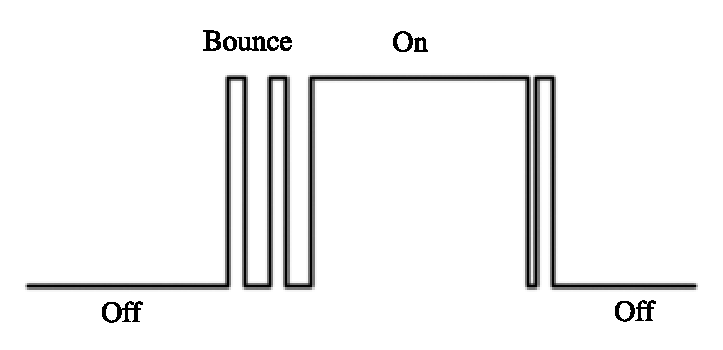
\includegraphics[width=0.45\textwidth]{img/Bounce.eps}
  \caption{Bounce effect in buttons.}
  \label{fig:bouncing}
\end{figure}
The fluctuations may cause several false press and release events. To solve this problem, so-called de-bouncing is applied. This technique, measures the state of the signal several times, with each measurement separated by a short delay. A button press event is only generated if all measurements confirm that the button is pressed.

The algorithm implemented in the generic component \emph{DebouncedButtonC} waits for an interrupt, which notifies about a button state change, and then, probes three more times during a 60ms interval. All edge cases were taken care of. This includes false alarms, when after the interrupt, the state doesn't seem to be changed or when the state changes just before we rearm the interrupt.

This component was made generic, because Chronos has five buttons. In Figure~\ref{fig:UpButtonC} we present the structure of one of them. All others are supported in the same way.

\begin{figure}[h]
  \centering
  \includegraphics[width=0.85\textwidth]{diagrams/UpButtonC.eps}
  \caption{The \emph{UpButtonC} abstraction.}
  \label{fig:UpButtonC}
\end{figure}
The \emph{HplMsp430GeneralIOC} and the \emph{HplMsp430InterruptC} are TinyOS library components that give access to GIO pins for MSP430 MCUs. The first provides access to pin state control, which allows for setting or probing the value of a pin. The second allows for arming interrupts that fire when the state of a pin changes. This is used to discover when a button is pressed.

An application using a button can either check the button's state with the \emph{Get} interface or be notified about a change through the \emph{Notify} interface. Finally note that thanks to the independency of the button implementations, it is possible to recognize press combinations.

\subsection{Buzzer}

Chronos has a built-in sound emitting device, called the buzzer. It can emit beeps typical to alarm clocks.

The buzzer isn't connected directly to an IO pin, as Figure~\ref{fig:chronos_schema} would suggest. Instead, an IO pin triggers a transistor that closes the buzzer's circuit. A 47k$\Omega$ resistor ensures that only a minimal current is drawn from the MCU. Drawing large currents from IO pins is not recommended and can be harmful.

The IO pin needs to be set high, to close the buzzer's circuit, which, in turn, moves its membrane one way. Cutting the current moves the membrane back. This way, a rectangular signal from the IO pin is transformed into sonic waves. The frequency of the waves is the same as the frequency of the signal.

We started the driver implementation by trying to actively generate this rectangular wave. Interestingly, we found that the resulting beeps had artifacts. The tone wasn't clear. As it turned out, after disabling the interrupts the artifacts disappeared. What we heard, were interrupts firing and interleaving with the signal. This is the first time that we've been able to observe interrupts using human senses!

Even though active signal generation with interrupts disabled is hardly a good solution, we had neither need nor time to investigate other options. Therefore, we left the improvement of the implementation for future work. The root component of the buzzer driver is \emph{BeeperC}, depicted in Figure~\ref{fig:buzzer_c}.
\begin{figure}[h]
  \centering
  \includegraphics[width=0.9\textwidth]{diagrams/buzzer_c.eps}
  \caption{The buzzer driver structure.}
  \label{fig:buzzer_c}
\end{figure}
It uses \emph{BusyMicroWaitC} to generate a wave form. This is more wasteful than setting an alarm, but also much more precise, and precision is necessary to generate a clear tone. \emph{BeeperC} provides a simple interface that enables sounding a single beep or a whole \emph{Power Rangers} style hail signal\footnote{It is used in the Zordon demo application.}. Though this hail is long, interrupts are only disabled while each distinct sound is emitted. This allows for processing all pending interrupts between the sounds.

The support for the Buzzer, the LCD display, and the buttons allow Chronos to be a standard hand watch. Let's now discuss more advanced features that distinguish it form such devices.

\subsection{The CC1101-based radio module}

The CC1101 is a radio transceiver chip made by Texas Instruments. Among others, it is used in the SOWNet's \cite{G-Node} wireless sensor node, depicted in Figure~\ref{fig:gnode}. This platform is important to us, for two reasons. Firstly, a large testbed of G-Nodes has been deployed in our faculty (see \cite{MM}). Secondly, TinyOS was ported to G-Node by SOWNet's developers. This ensures the quality of the code and an ongoing support. Moreover, the port was released on a license similar to that used in the rest of TinyOS, allowing for royalty-free use and even modification.

\begin{figure}[h]
  \centering
  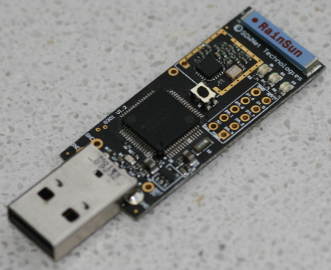
\includegraphics[width=0.4\textwidth]{img/gnode.jpg}
  \caption{The SOWNet's G-Node.}
  \label{fig:gnode}
\end{figure}
We took the position that further research would be enhanced if communication was possible between the watches and the G-Nodes\footnote{This way our testbed would become one of the largest academic deployment of wireless sensor nodes in the world, consisting of over 220 devices.}. Even though the CC1101 radio core used in G-Nodes is a stand alone product, recently it was also built into the members of the CC430 family of MCUs, hence the two are hardware-compatible. Adding this to the fact that we were time constrained, we decided to adapt the G-Node's radio stack implementation, so that it could run on Chronos. Having the same code on both types of devices provides maximum compatibility. We also made sure that this step was legitimate by complying with the license restrictions.

We do not present the detailed structure of the radio stack here because of its complexity. Instead we focus on our porting efforts. For details on the design of the ActiveMessage communication model please refer to \cite{BHC}, \cite{TEP116} and \cite{TEP126}.

The fundamental difference between the external CC1101 core and the built-in one lies in the way they communicate with the MCU. The standalone chip uses the SPI bus and some additional signal lines, while the internal core accepts commands through a register based interface. As we expected, almost everything else remains the same. It seems that TI has embedded the radio core into an MCU design and changed only the command interface.

Our modifications thus followed the same pattern. We removed all SPI related code from the HAL layer. Then, we changed the HAL code, to send all commands through appropriate registers. At that point, we were only missing the interrupts and status signals that were previously generated from signal lines coming from the radio chip. Interrupts were, however, easy to replace with native ones, sourced directly from the built-in core, while status signals could be read from registers via query commands (or in some cases, even directly). In the end, we cleaned up the code by removing some redundant definitions and adding comments documenting each command. Our final impression is that the built-in core is easier to manage than the external one.

The bulk of those changes were applied to the \emph{HalChipconControlP} module, which drives the radio core. It provides the \emph{HalChipconControl} interface, which can be used for low level radio operation. It gives the user precise control over transmission and reception, which might be necessary in some more sophisticated communication protocols.

During the development we encountered some serious difficulties. The biggest delay was caused by an elusive bug we introduced in the code. Namely, we called an interface function, rather than a local one that wrapped it. They had similar names, which made the difference difficult to notice. The function's purpose was to read the radio core's inner registers. However, without the use of the wrapper, a few of them were read incorrectly. This caused the radio to fail under some conditions, while working normally most of the time. We spent literally weeks, trying to find the source of the instability. At that point, we only had the LCD display to view the state of the watch and it only supported displaying numbers. Seeing that this was getting us nowhere, we started working on enabling the TinyOS \emph{printf} library. It helped a lot, allowing us to ascertain the exact condition at which the radio failed. After some investigation, we found that it happened during, seemingly harmless radio core register read. Finally, we noticed the misuse. That error was simple, but also very difficult to track down.

Another issue we had concerned G-Node interoperability. After porting G-Node's radio stack to Chronos, we expected that both would be able to communicate with each other. This wasn't the case though. We made sure that the transmission speeds matched, checked that G-Nodes were able to communicate among themselves and that Chronoses could do the same, but still they couldn't be mixed together. Finally, we found that the problem was rooted in the \emph{support/make/chronos.target} file. Namely, it didn't contain any definition of the \emph{DEFAULT\_LOCAL\_GROUP} constant. This caused the build system to impose a default value, different from the G-Node's default. In effect G-Node and Chronos used different values for the \emph{DEFAULT\_LOCAL\_GROUP}, and nodes from different local groups ignore each other's messages. We fixed it by defining the \emph{DEFAULT\_LOCAL\_GROUP} as empty, in the mentioned file. Interestingly, an empty environment variable is treated differently than an undefined variable. Some may view this as obvious, yet it caused us problems all the same.

Afters solving all problems, we've investigated the maximum length of the data that can be sent in one packet. In TinyOS this value is configured with the \emph{TOSH\_DATA\_LENGTH} constant. The size of the radio internal transmission/reception queue is 64 bytes. 11 are used for TinyOS packet header and 3 for the footer. This leaves 50 bytes for the payload. Interestingly, the radio seems to work even with this value set to 52. However we strongly recommend never to exceed 50.

\begin{figure}[h]
  \centering
  \includegraphics[width=1.0\textwidth]{diagrams/am_sender_c.eps}
  \caption{Overview of the \emph{AMSenderC} abstraction.}
  \label{fig:am_sender_c}
\end{figure}

Finally, note that the radio stack can be used through the interfaces provided by the \emph{ActiveMessageC}\footnote{This is an example of the Placeholder design pattern.} configuration. This however becomes less convenient if multiple message types are to be be sent and received. In such cases it is better to use the \emph{AMSenderC} generic component, shown in Figure~\ref{fig:am_sender_c}, which can be parametrized with the message type. It sends and receives only messages that have a particular id. At most one instance of this component in the system can use a given id, removing the risk of collisions. Moreover it provides a one-element message queue, which helps in arbitration between users of different message types, allowing them to forget about each others existence. For an excellent tutorial on how to use the radio stack in an application, see \cite{MoteToMote}. Also note that using the \emph{Low Power Listening} technique, supported by the radio stack, dramatically reduces power consumption. More on that can be found in \cite{LowPowerApps}.


\subsection{Centralized port management}

We noticed a bad practice TinyOS developers. Too often, various configurations, directly connect enumerated ports to components, like for example \emph{IO.Port31 -> SPI.ChipEnable}. This hides dependencies, making code much more difficult to understand and reuse. Moreover, experiments and modifications require a detailed review of schematics and datasheets to track the connections. Pin numbers neither indicate the MCU-side special function, nor the function of the pin on the other end. Continuing the above example, we don't know which peripheral device Port31 enables and if this port can even support the peripheral on the MCU side. It is difficult to ensure that one got the connections right, especially when they need to run crossover, like UART's TX and RX.

This matter becomes even more problematic in the case of CC430 MCUs, because they can dynamically reassign pin special functions. Moreover, doing this incorrectly blocks the ability of further port-mapping changes until the device is restarted. Thus, one faulty piece of code can break completely correct code. A source of such an error is difficult to track.

These issues lead to two conclusions. Firstly, it would be better to give ports mnemonics, describing their real purpose and use these abstract names in configurations. Secondly, port mapping should be done in one place. As both solutions need to be kept in sync, we believe that the best option is to join them, forming a centralized port management abstraction. Our implementation of this abstraction in Chronos took shape of the \emph{PlatformPortmapC} component. It provides IO pin interfaces named with the MCU pin special functions and ones representing the remote sides of the connections. Figure~\ref{fig:platform_portmap_c} shows the simplified structure of this component. Here it only provides access to two ports. \emph{CMA3000CSB} represents the accelerometer's chip-enable and \emph{CMA300MOSI} is its master-out slave-in SPI line. The \emph{UCB0SIMO} is a name of the special function assigned to the pin. It means that it acts as the slave-in master-out line, when USCI\_B0 submodule is configured to be an SPI interface. This function is assigned to Port16 by the \emph{PlatformPortmapP} module, which is responsible for the special function remapping. PortJ is somewhat special. We had to add support for it to the  \emph{HplMsp430GeneralIOC} and its pins cannot have special functions assigned.

\begin{figure}[h]
  \centering
  \includegraphics[width=0.9\textwidth]{diagrams/platform_portmap_c.eps}
  \caption{The centralized port management in Chronos. (simplified)}
  \label{fig:platform_portmap_c}
\end{figure}

Figure~\ref{fig:} show how the accelerometer driver can use the \emph{CMA3000CSB} and the USCI\_B0 driver can use \emph{UCB0SIMO}, rather than concrete numbered pins.

\begin{figure}[h]
  \centering
  \includegraphics[width=0.9\textwidth]{diagrams/portmap_clairty.eps}
  \caption{Advantage of using the centralized port management.}
  \label{fig:}
\end{figure}
Notice that each component connects to a pin with a name, characteristic to this component. The USCI\_B0 driver, doesn't have to know that the line leads to the accelerometer. And similarly, the accelerometer driver doesn't have to know the exact number of the pin connected to the chip-enable line. All information about the actual circuit board connections is hidden in \emph{PlatformPortmapC}. This gives potential for code portability. Another MCU from the CC430 family would only need an updated \emph{PlatformPortmapC} file to support the accelerometer\footnote{However, rarely is it that simple. Often one more level of indirection is needed to achieve portability. See \emph{PlatformCMA3kD0C} component in Section \ref{ch:accelerometer}.}. Writing code for \emph{PlatformPortmapP} is also simplified because it only needs to realize mappings described in its parent configuration.

The solution described above is important for Chronos. All external connections, such as those in Figure~\ref{fig:chronos_schema}, use different hardware subsystems. This would not be possible without port management, because CMA3000-D01 and the USB debug dongle would have to share USCI\_A0.

\subsection{The serial connection support}

% through mspdebug bi-wire ?
% through radio packets ?

The serial port connection is the most reliable way for the MCU to communicate with a PC. It allows for relying packets between the tools on the PC and the radio mesh network. It also allows for receiving network activity logs to analyze the network operation. During the code development cycle, in turn, it enables printing messages from the MCU on a PC console, greatly reducing the debugging effort.

For Chronos, the best way to connect to a PC is to use the UART protocol in conjunction with the USB debug dongle. This protocol uses only two wires and is natively supported by the MCU hardware. There is, however a small hardware modification that needs to be done to the watch to make UART operational. The modification is described in detail in Appendix \ref{appendix:uart_pins}.

The UART, SPI and I2C are only protocols. They define how wires should be connected between devices, and what signals should be sent, to make the devices communicate. Each protocol, however, must first be implemented in either software or hardware. The CC430 MCUs provide such a hardware implementation for all three protocols in form of a submodule called USCI. It can be configured to communicate using one of the protocols and send the signals with special MCU pins (i.e. UCA0TXD, UCA0RXD). The MCU can send its data, through USCI, by writing bytes to special registers, and by handling its interrupts. These details are, however, handled by libraries, which provide higher-level communication interfaces. In Chronos we use the USCI submodule for serial communication with PC and on-board peripherals.

Let us analyze how the serial stack is organized in TinyOS, by looking at the main component of the \emph{tos/lib/serial} library, \emph{SerialActiveMessageC}. The component, a configuration to be precise, depicted in Figure~\ref{fig:serial_active_message_c}, provides interfaces  similar to those of the radio stack.
\begin{figure}[h]
  \centering
  \includegraphics[width=0.6\textwidth]{diagrams/serial_active_message_c.eps}
  \caption{The \emph{SerialActiveMessageC} component. (simplified)}
  \label{fig:serial_active_message_c}
\end{figure}
We do not delve into them and refer the reader to \cite{TEP113} for details. The configuration relies on \emph{SerialDispatcherC}, depicted in Figure~\ref{fig:serial_dispatcher_c}, to provide \emph{SubSend} and \emph{SubReceive} functionality.
\begin{figure}[h]
  \centering
  \includegraphics[width=0.75\textwidth]{diagrams/serial_dispatcher_c.eps}
  \caption{The \emph{SerialDispatcherC} component. (simplified)}
  \label{fig:serial_dispatcher_c}
\end{figure}
In \emph{SerialDispatcherC}, there are three components involved in packet preparation and transmission over a byte stream medium, but at the bottom lies the most important for us: \emph{PlatformSerialC}. It provides \emph{UartStream} for byte transmission and \emph{StdControl} for turning the connection on and off. Having this component is the key for a platform to support the serial communication. As the ports were already configured to the state shown in Figure~\ref{fig:chronos_schema} by \emph{PlatformPortmapC}, to enable serial communication on Chronos, we only needed to get the USCI\_A0 module act as an UART driver and provide an interface to it.

After some investigation, we found the \emph{tos/chips/msp430/x2xxx/usci} library that supports USCI modules of some MSP430 MCUs. Most importantly, it configures USCI and provides the \emph{UartStream} interface that we need. It isn't, however, directly compatible with Chronos. There are some differences in register naming and interrupt sources, but not too big and we managed to adapt it for our purposes. We didn't find a way to modify the library itself without breaking the other supported platforms. The necessary modifications were needed deep inside the library, hence inserting them would require a major refactoring of the entire library. Therefore instead, we copied the library locally to the Chronos platform and changed what we needed: a crude solution, but effective.

\begin{figure}[h]
  \centering
  \includegraphics[width=0.52\textwidth]{diagrams/platform_serial_c.eps}
  \caption{The \emph{PlatformSerialC} component.}
  \label{fig:platform_serial_c}
\end{figure}

Figure~\ref{fig:platform_serial_c} presents the \emph{PlatformSerialC} component, that was the result of our work. The \emph{Msp430Uart0C} is the root component of the USCI library. It uses the \emph{Msp430UartConfigure} interface to retrieve the UART configuration parameters and provides the \emph{Resource} interface, which is a part of the integrated concurrency and power management control mechanism used to gain access to the serial line. \emph{ChronosSerialP} only stores the aforementioned configuration parameters. The rest is done behind the scenes, the net result is that the \emph{SerialActiveMessageC} component is available. The \emph{tos/lib/printf} library uses it directly and thus, we also gained the ability to print messages on, PC console. Details on how to use this library are described in Appendix \ref{ch:prog_env}.

\subsection{The accelerometer}
\label{ch:accelerometer}

CMA3000-D01 is the accelerometer chip installed in Chronos. It enables measuring the acceleration that the watch is subject to at any given moment. This includes the Earth's gravity, which allows for estimating the device's orientation in space. In addition using accelerometer readings, some human activities can be recognized. The CMA3000-D01 chip has three modes of operation. In the measurement mode, it sends a continuous stream of samples at a preconfigured rate. In the motion detection mode, the chip uses little energy, while readily detecting any motions exceeding preconfigured thresholds. Similarly, in the free fall detection mode, it notifies the MCU whenever acceleration readings fall below given thresholds. Overall, such sensor enables creating some very interesting applications.

However, this particular chip wasn't supported in TinyOS. This created an opportunity for us, to design its device drivers from scratch. During our work, we closely abided by the recommendations of the Hardware Abstraction Architecture, therefore this code is our best example of its use. We also made the driver platform independent in the same way that \emph{SerialActiveMessageC} is. The platform only needs to provide a proxy component bridging its communication lines with the driver code.  This connection is realized by the \emph{PlatformCMA3kD0C} configuration, shown in Figure~\ref{fig:platform_cma3kd0_c}.

\begin{figure}[h]
  \centering
  \includegraphics[width=1.0\textwidth]{diagrams/platform_cma3kd0_c.eps}
  \caption{The bridge between the platform and the accelerometer driver.}
  \label{fig:platform_cma3kd0_c}
\end{figure}
The \emph{PlatformCMA3kD0C} component must be implemented by the user of the library. Most importantly, this component must provide the \emph{SpiPacket} interface that allows for communicating with the CMA3000-D01 chip, along with the \emph{Resource} interface used to secure exclusive access to the SPI bus. In addition, it should provide interfaces that give control over the IO lines that connect the MCU and the chip. These include the chip-select line, chip-power line and the chip-to-MCU interrupt line. While it is possible to use the accelerometer without control over their signals, doing so would reduce its functionality. In the Chronos platform, the \emph{PlatformCMA3kD0C} component instantiates the \emph{Msp430SpiB0C} to obtain the \emph{SpiPacket} interface. \emph{Msp430SpiB0C} originates from the same library that is used to support the serial connection. As shown in Figure~\ref{fig:chronos_schema}, the \emph{PlatformPortmapC} connects the USCI\_B0 subsystem to the accelerometer, therefore \emph{Msp430SpiB0C} indeed realizes the desired connection. The IO pin interfaces are sourced from the \emph{PlatformPortmapC} directly\footnote{Well almost, because the \emph{Msp430GpioC} adapter is used to convert the \emph{HplMsp430GeneralIO} interface to a platform independent \emph{GeneralIO}.}.

The interfaces provided by the proxy component are used in the Hardware Presentation Layer of our driver. Its members can freely instantiate and internally depend on the \emph{PlatformCMA3kD0C} component, because from the outside it is completely platform independent.
\begin{figure}[h]
  \centering
  \includegraphics[width=1.0\textwidth]{diagrams/hpl_cma3kd0_c.eps}
  \caption{The HPL of the accelerometer driver.}
  \label{fig:hpl_cma3kd0_c}
\end{figure}
Figure~\ref{fig:hpl_cma3kd0_c} shows all the components comprising the HPL. The most important abstraction is the accelerometer register access. It originates from the way the accelerometer is controlled. There is only one frame, that can be sent to it through the SPI. This frame contains a register address, a read-write bit and a data byte. If the bit indicates a write, than the accelerometer sets the specified register to the specified value and sends an answer frame, though it's not relevant in this case. It becomes relevant, however, if the bit was set to read, in which case, the answer caries the register value.

The main responsibility of the HPL is to abstract this mechanism, to allow for simple register modifications. We achieve this by splitting each register into the smallest meaningful portions, that we call subregisters, like the interrupt-enable bit or the 3 bits that configure the currently set accelerometer mode. HPL provides a simple interface that allows to set the value of a specific subregister, without changing the value of the whole register. Technically this violates the HPL contract because we must store some state in the components, but that's only necessary due to the split-phase nature of SPI communication. Had it been synchronous, stack variables would suffice. More important than the lack of state is the primary purpose of the HPL, which is to provide a clean interface to the hardware and we definitely succeeded in that.  The second thing that HPL does is the one time configuration of the interrupt line. Further responsibility for interrupt processing is left for the HAL, though.

Another responsibility of HAL is concurrency. Typically, there are more than one entity wanting to use the accelerometer. Moreover, one entity may wish to use two of its functions consecutively. It could, for example, first wait for a motion and, after motion is detected, activate the more costly measurement mode. The HPL drivers don't have any notion of concurrency, though. Trying to make a second register access before the first one finises, yields unpredictable results. Therefore, we introduced the \emph{HalCMA3kD0OwnershipC} component, depicted in Figure~\ref{fig:hal_cma3kd0_ownership_c}.
\begin{figure}[h]
  \centering
  \includegraphics[width=0.85\textwidth]{diagrams/hal_cma3kd0_ownership_c.eps}
  \caption{The integrated concurrency and power management for the accelerometer.}
  \label{fig:hal_cma3kd0_ownership_c}
\end{figure}
It uses the mechanism demonstrated in Section \ref{ch:concurrency_and_power} to arbitrate the access to HPL and the CMA3000-D01 chip itself. This is done via the \emph{Resource} interfaces it provides. Each user of HPL must first request and be granted access to it. When the device isn't used, it is left under the control of the default owner, which is the \emph{HalCMA3kD0PowerManagerP} component. It is responsible for powering down the device, but it does so in an optimized manner. Instead of immediately cutting the power, it delays, waiting for a next user. This prevents an inefficient flickering behaviour when the accelerometer would have been turned on and off with a high frequency. Now this frequency is bound by the inverse of the delay period. Note, however, that the default owner also requests and holds access to the SPI bus, so the delay shouldn't be too long.

This concurrency control and HPL form the foundation for a higher-level accelerometer abstraction implemented in the Hardware Abstraction Layer. It strives to expose most of the device's capabilities to ensure a maximal efficiency and performance. The design is organized around the three accelerometer operation modes. Each is supported by a separate HAL component that provides an interface specific to its mode. However, the broad configuration possibilities can be a flaw in more casual use or when platform independence is more important. Therefore, the Hardware Independence Layer also provides components that wrap HAL, configure the accelerometer to safe default values provide easy to use and portable interfaces. The code supporting each accelerometer mode is similar. Therefore, we focus only on how the measurement mode is implemented, because it sufficiently covers the most important concepts.

Samples are always read by accessing three registers containing the components of the acceleration vector. In the measurement mode, however, the accelerometer not only tries to produce readings at a constant rate, but also notifies the MCU about readiness of a new sample, by changing the signal on the interrupt line. The MCU configures its GIO to monitor this line and fire an interrupt when a change is detected. This allows for reading the sample as soon as it's ready, without wasteful pooling. Figure~\ref{fig:hil_accel_stream_c} shows the components supporting the measurement mode.
\begin{figure}[h]
  \centering
  \includegraphics[width=0.8\textwidth]{diagrams/hil_accel_stream_c.eps}
  \caption{The support for continuous acceleration measurements.}
  \label{fig:hil_accel_stream_c}
\end{figure}

The bulk of the logic is implemented in the \emph{HalCMA3kD0ContinousReadsP} module. It takes care of accelerometer configuration, handling the interrupts, and reading the samples. The \emph{HalCMA3kD0ContinousReadsC} makes the necessary connections and hides unnecessary details. On top of it, the HIL component is built. The \emph{HalCMA3kD0ContinousReads} interface enables configuring both the rate at which samples are taken and the precision scale. \emph{HilAccelStreamP} hides these details, by setting the frequency to 40Hz and the scale to the maximum of 8g. It also requests the resource behind the scenes, so that the user can receive samples purely by the means of the simple \emph{Notify} interface.

The whole HAA structure of the driver is presented in Figure~\ref{fig:accel_haa_structure}.
\begin{figure}[h]
  \centering
  \includegraphics[width=1\textwidth]{diagrams/accel_haa_structure.eps}
  \caption{HAA structure of the accelerometer driver.}
  \label{fig:accel_haa_structure}
\end{figure}

\subsection{Persistent storage}

Many applications, need non-volatile memory to perform their functions. Therefore, we decided that the Chronos platform must provide some form of persistent storage. We tried to add support for it, however, this proved more difficult than anticipated and we haven't succeed yet. This section describes how persistence is supported in TinyOS. We also draw lessons from our flawed design and lay plans for future work.

There is a well defined set of HIL interfaces meant to support non-volatile memory in TinyOS. The authors of \cite{TEP103} selected the three most common use cases, and, for each, designed a custom abstraction. The first is represented by the \emph{ConfigStorageC} component, and is used to store application's configuration, which usually is a set of small numeric values. The second, allows for the storage of large binary objects, through the \emph{BlockStorageC} configuration, which provides interfaces for efficient block reads and writes. The third is used to store logs. The \emph{LogStorageC} component ensures consistency of the records and supports circular logging.

However, the implementation of these interfaces was left fully in the discretion of the programmer, mainly due to a large variety of flash chips and performance considerations. The authors recommend that each chip should have its own customized driver implementation and they do have a point, because Chronos has no flash chip at all. Nevertheless, we decided that persistent storage is very important and must be supported somehow. Fortunately, it is possible to write to the MCU's internal flash memory runtime. Therefore, we can use a part of the program memory for application storage needs.

The flash memory of the watch is organized into three categories. The main program memory has 32KB and is divided into 512-bytes long segments. There is also the so called info memory, that has 4 segments, each 128 bytes long, and is meant specifically for configuration data. The last type of memory is used by the bootstrap loader and consists of 4 segments, each 512-bytes long. Memory segmentation is important, because segment is the minimal unit that can be erased. An erase sets all bits in a segment to 1. Writes can clear bits to 0, but can never set a 0 to a 1. This is an important constraints when dealing with flash memory in low-power MCUs.

An additional difficulty in Chronos is the fact that any write to the flash memory completely halts the MCU. This means that writes should be done in short bursts, to avoid delaying any pending tasks. Finally, as far as we know, the mass erase done during reprogramming, clears the main memory, but leaves the info and bootstrap loader segments intact. A subtlety that we completely disregarded in our first approach to the driver implementation.

We started by working out the low level details of memory writing and erasing. The resulting component structure is shown in Figure~\ref{fig:hal_cc430_internal_flash_c}.
\begin{figure}[h]
  \centering
  \includegraphics[width=0.8\textwidth]{diagrams/hal_cc430_internal_flash_c.eps}
  \caption{The flash segment abstraction.}
  \label{fig:hal_cc430_internal_flash_c}
\end{figure}
It is organized around the concept of segments, being independent portions of the memory. This idea isn't bad, because it's convenient to assume that the whole segment can always be erased. The problem, however, is that this approach makes no distinction between segments. Segments vary in size and the mass erase persistence, but higher layers can not rely on these properties. Another issue is that the \emph{writeBuffer} operation was made synchronous which introduced lengthy tasks. Finally, the HPL has too much logic in it, making it effectively a HAL component. The code accesses registers directly, creating the exact clutter that HPL and HAL separation was supposed to avoid. Overall, the internal flash HAL creates a leaky abstraction that tries to hide too many details, making subsequent use more difficult.

The HIL layer, in turn, is presented in Figure~\ref{fig:log_storage_c}.
\begin{figure}[h]
  \centering
  \includegraphics[width=0.8\textwidth]{diagrams/log_storage_c.eps}
  \caption{The HIL components of the driver.}
  \label{fig:log_storage_c}
\end{figure}
It consists of two bulky components, \emph{HilCC430LogReadWriteP} and \emph{HalCC430CircularStorageC}, which are tightly coupled.
Multiple times we had to adjust the interface connecting them to implement their logic. The lacking lower layer overly complicates the circular storage component. Moreover, note that there is no trace of any concurrency management, which is required by the specification. At that time, we understood little of how TinyOS handles these issues. In practice the implementation worked poorly and eventually we decided to abandon it.

To avoid the above mistakes, we plan to employ test-driven development during our second approach. Very recently this was made possible by \cite{TOSMock}. This technique tends to produce smaller, more loosely coupled components with better interfaces, and helps find programming errors early in the development cycle. These are the virtues that the current implementation lacks.

%\subsection{The temperature and pressure sensor}
%Chronos has SCP1000-D11 chip, which measure absolute pressure and temperature.
%The sensing element is a silicon wafer that is locally thinned to form a pressure sensitive diaphragm.
%
%The chip provide four reading modes: high resolution, high speed, ultra low power and low power with external trigger.
%First three of them continuously provide new data, while the last one refreshes data after the update is triggered.
%In every mode the temperature and pressure is available for each measurement.
%The chip communicate with MCU using $I^2C$ interface. 
%However, in some parts of documentations this interface is called TWI to avoid trademark issues.
%
%The implementation provide four components: 
% diagrams does not work :-(







% to enable wrapped line navigation:
% map j gj
% map k gk

% vim settings:
% vim: set nonumber:
% vim: set spell:
% vim: set linebreak:
% vim: set wrap:
% vim: set textwidth=0:
% vim: set fo+=t:
